\section{Erstellung eines Datenkonzepts} \label{Erstellung eines Datenkonzepts}
Im nun folgenden Kapitel werden die zuvor in den Kapiteln \ref{Analyse Datenbestaende} und \ref{Stand der Technik} beschriebenen Metadaten der einzelnen Systeme zu einen umfassenden Datenkonzepts zusammengefasst. Dieses Konzept bildest die Grundlage zur Speicherung in einem \ac{DMS}.

F\"ur die grafische Darstellung des Metadatenmodells wurde eine UML-Darstellung gew\"ahlt, wobei Klasse eine Datensammlung dartstellt. 

Es wird explizit darauf hingewiesen, dass die Darstellung kein Klassendiagramm nach UML im eigentlichen Sinn ist und somit von der von der vorgeschriebenen Darstellungsform abgewichen wurde.

Attribute, welche sich direkt in der Sammlung befinden sind ohne besondere Kennzeichnung einfach dargestellt. Andere Attribute, welche wiederum auf eine Datensammlung verweisen, sind mit dem jeweiligen Verweistyp gekennzeichnet. Zus\"atzlich wird mit Hilfe der Hintergrundfarbe sichtbar gemacht, in welchem Package sich die Datensammlung befindet. 

Verweise sind zus\"atzlich \"uber Pfeile gekennzeichnet, an welchen die Kardinalit\"at zu finden ist.

Um in der Arbeit eine \"Ubersicht zu geben, werden die Packages einzeln beschriebenen. Eine gesamte \"Ubersicht des Diagramms ist auf dem der Arbeit beiliegenden Datentr\"ager zu finden.

\subsection{FADO Metadaten}\label{FADO Metadaten}
In Abbildung \ref{Fado Modell} ist der erste Ausschnitt des Datenmodells zu sehen, welcher das Package \texttt{FADO Metadaten} zeigt.

Die Metadaten sind in vier Datensammlungen zusammengefasst, die wichtigte ist \texttt{FADO Metadaten}. In dieser Dammlung sind Dokument\"ubergreifende Metadaten gesammelt, welche von allen FADO-Dokumenten verwendet werden. Zum Teil k\"onnen hier alte Attribute wie Unsichtbar oder Ausblenden wiedergefunden werden. Zum Teil haben die Namen der Attribute sich aber such ge\"andert, warum eine Tabelle mit dem Mapping zwischen alten und neuen Namen im Abschnitt \ref{Metadatenmapping} zu finden ist.

Die drei Datensammlungen \texttt{FADO Urteil}, \texttt{Forschungsvorhaben} und \texttt{Bibliographische Angaben} sind die jeweiligen Hauptdatensammlungen der betrachteten Dokumente \texttt{Urteile}, \texttt{Forschungsvorhaben} und \texttt{Berichte}.

Attribute, welche farblich hinterlegt sind, stellen wie schon erw\"ahnt verweise zu anderen Datensammlungen dar. Im vollst\"andigen Diagramm, werden diese Verweise zus\"atzlich durch Pfeile realisiert, welche die entsprechenden Kardinalit\"aten anzeigen.
\begin{figure}[!ht]
\centering
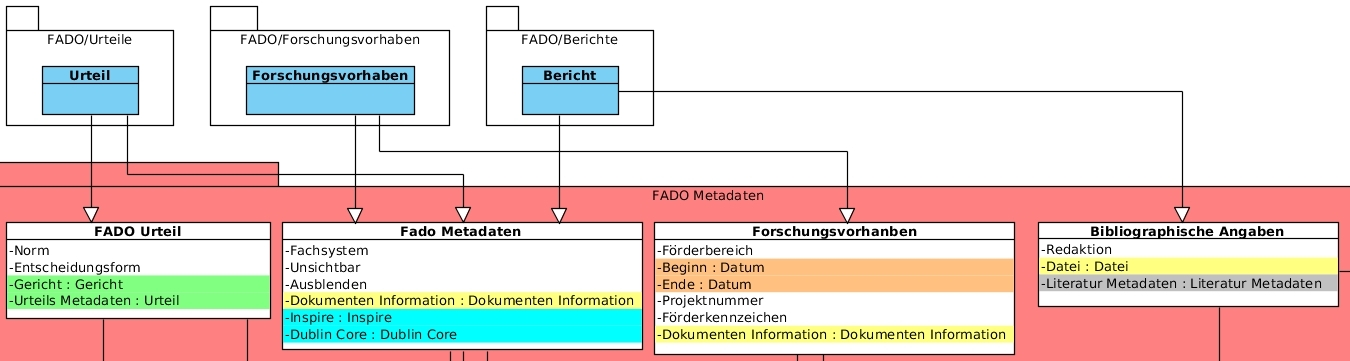
\includegraphics[width=16cm]{Bilder/Datenmodell/FADO-Metadaten.jpg}
\caption{FADO Metadaten}
\label{Fado Modell}
\centering
\end{figure}

\FloatBarrier
\subsection{DRS Metadaten / Bildarchiv Metadaten}\label{DRS Bildarchiv Metadaten}
Die Abbildung \ref{DRS und Bildarchiv Modell} zeigt die Datensammlungen des \ac{DRS} und des Bildarchives. Hier sind wie schon in \ref{Fado Modell} Abbildung die obersten Datensammlungen zu sehen, welche zum einen eigene Attribute enthalten und zum anderen wieder auf untergeordnete Datensammlungen verweisen. 

Das Mapping zu den Metadaten ist im Abschnitt \ref{Metadatenmapping} zu finden.
\begin{figure}[!ht]
\centering
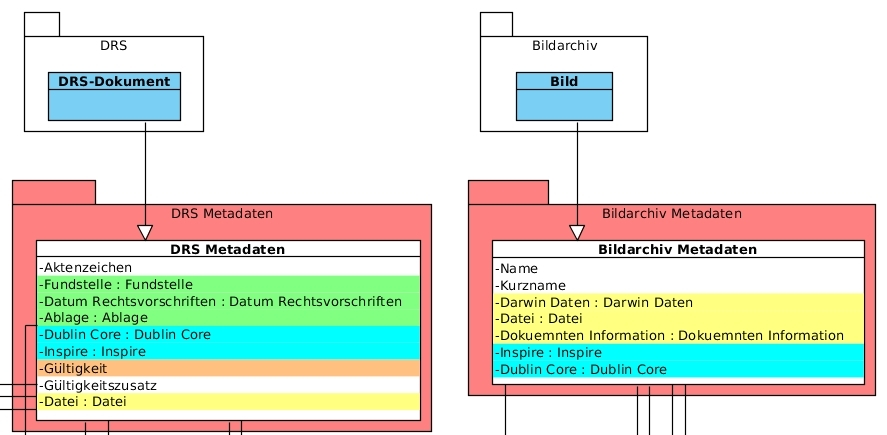
\includegraphics[width=12cm]{Bilder/Datenmodell/DRS-Bildarchiv-Metadaten.jpg}
\caption{DRS und Bildarchiv Metadaten}
\label{DRS und Bildarchiv Modell}
\centering
\end{figure}

\FloatBarrier
\subsection{ICT-ENSURE Metadaten}\label{ICT-ENSURE Metadaten}
Abbildung \ref{ICT-ENSURE Modell} zeigt die Hauptdatensammlungen der Metadaten f\"ur \ac{ICT-ENSURE} Metadaten. Eine Besonderheit ist hier, dass die Datensammlung in geteilt ist und zwar in \texttt{Artikel Metadaten}, welche die Metadaten zu einem Artikel enth\"alt und in \texttt{Konferenz}, in der die Metadaten zu einer Konferenz zu finden sind.

Alle farbig hinterlegten Verweise sind in den nachfolgenden Abschnitten genauer erkl\"art und das Mapping zwischen alten und neuen Namen ist im Abschnitt \ref{Metadatenmapping} zu finden.
\begin{figure}[!ht]
\centering
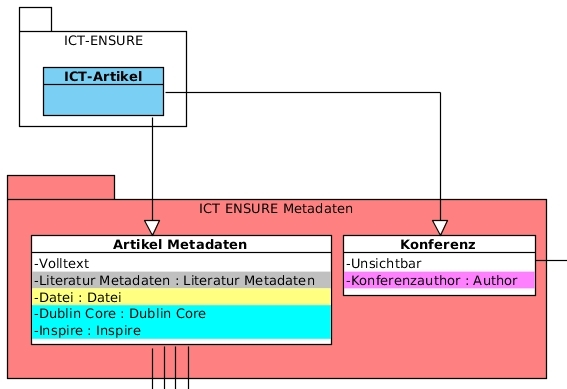
\includegraphics[width=8cm]{Bilder/Datenmodell/ICT-ENSURE-Metadaten.jpg}
\caption{ICT-ENSURE Metadaten}
\label{ICT-ENSURE Modell}
\centering
\end{figure}

\FloatBarrier
\subsection{Untergeordnete Datensammlungen}
In den nun folgenden Abschnitten, werden die eben in den Abbildungen \ref{Fado Modell} bis \ref{ICT-ENSURE Modell} farbig hinterlegten Datensammlungen mit ihren Attributen genauer beschrieben. 

\subsubsection{Gerichtbarkeit}
Im Package Gerichtbarkeit, welches in Abbildung \ref{Package Gerichtbarkeit} zu sehen ist, sind alle Datensammlung zusammengefassen, welche f\"ur Gerichtliche Urteile, Beschl\"usse oder Richtlinien wichtig sind zusammengefasst.

Die Datensammlungen \texttt{Gericht} und \texttt{Urteil} werden wie in Abbildung \ref{Fado Modell} zu sehen in der Datensammlung \texttt{FADO Urteil} verwendet.

Die Datensammlung \texttt{Gericht}, stellt wie der Name schon sagt ein Gericht dar. Hierbei enth\"alt sie die Attribute \texttt{Standort} und \texttt{Art}. Im Attribut \texttt{Standort}, wird der Standort des Gerichts und im Attribut \texttt{Art} die Art, wie zum Beispiel "`Oberlandesgericht"' festgelegt. So ergibt sich f\"ur ein Gericht der Datensatz aus Standort und Art mit dessen Hilfe ein Datum nach der Art "`Oberlandesgericht Karlsruhe"' gebildet werden kann.

Der Datensatz Urteil enth\"alt die schon analysierten Attribute, welche das \ac{FADO}-System verwendet. Die Attribute \texttt{Vorgericht} und \texttt{Nachgericht} verweisen wiederum auf ein Gericht, wie es eben beschrieben wurde. Das Erscheinungsdatum enth\"alt eine Datensammlung des Typs \texttt{Datum}, welche im Abschnitt \ref{Grundlegenden Daten} genauer beschrieben ist.

\texttt{Fundstelle}, \texttt{Datum Rechtsvorschriften} und \texttt{Ablage} sind Datensammlungen welche in der Sammlung \texttt{DRS Metadaten} vorkommen. Sie enthalten weitere Attribute zur Gerichtbarkeit, welche im \ac{DRS} verwendet werden. (siehe Abschnitt \ref{DRS Bildarchiv Metadaten})

Eine Fundstelle hat die Attribute \texttt{Name}, \texttt{Jahr} und \texttt{Seite}, welche eine Fundstelle wie sie im \ac{DRS} wiedergegeben wird beschreiben. 

Alle Attribute der Datensammlung \texttt{Datum Rechtsvorschriften} verweisen auf ein Datum, welches im Abschnitt \ref{Grundlegenden Daten} genauer beschrieben ist.

Die Datensammlung \texttt{Ablage} enth\"alt weitere Attribute, welche das \ac{DRS} zur Beschreibung seiner Dokumente verwendet.

Das Mapping zu gegeben \"Anderungen in den Namen ist im Abschnitt \ref{Metadatenmapping} zu finden.
\begin{figure}[!ht]
\centering
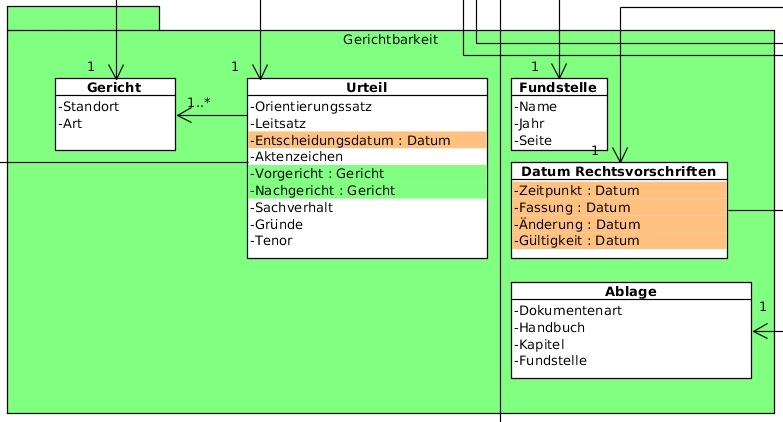
\includegraphics[width=10cm]{Bilder/Datenmodell/Package-Gerichtbarkeit.jpg}
\caption{Package Gerichtbarkeit}
\label{Package Gerichtbarkeit}
\centering
\end{figure}

\subsubsection{Bibliographie Metadaten}
Das Package \texttt{Bibliographie Metadaten}, in Abbildung \ref{Package Bibliographie} zu sehen, enth\"alt zwei Datensammlungen, welche sich mit der Beschreibung von Literatur befassen. 

Die Datensammlung \texttt{Literatur Metadaten} ist die eigentlich wichtige Sammlung und wird von den Datensammlungen \texttt{Bibliographische Angaben} (Abbildung \ref{Fado Modell}) und \texttt{Artikel Metadaten} (Abbildung \ref{ICT-ENSURE Modell}) verwendet.

Die Attribute \texttt{Seitenanzahl}, \texttt{Abstract}, \texttt{Reihe}, \texttt{Bandnummer}, \texttt{Beginn Seite} und \texttt{End Seite} sind selbsterkl\"arend und werden deshalb nicht genauer beschrieben. Das Attribut \texttt{Kapitel} verweist auf die gleichnamige Datensammlung und enth\"alt wiederum Angaben zum Kapitel.

Die Attribute \texttt{PublikationsID} und \texttt{Dokumenten Information} verweisen auf Datensammlungen im Package \texttt{Abstrakte Metadaten}, welche im Abschnitt \ref{Abstrakte Metadaten} genauer beschrieben sind.
\begin{figure}[!ht]
\centering
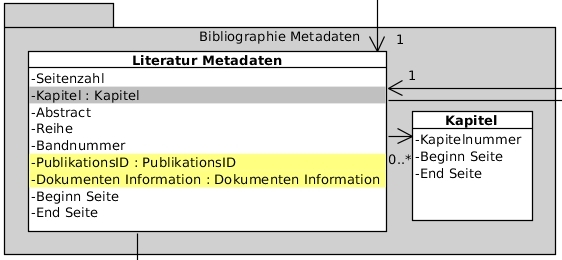
\includegraphics[width=8cm]{Bilder/Datenmodell/Package-Bibliographie.jpg}
\caption{Package Bibliographie}
\label{Package Bibliographie}
\centering
\end{figure}

\subsubsection{Abstrakte Metadaten}\label{Abstrakte Metadaten}
\texttt{Abstrakte Metadaten} ist ein Package, welches Datensammlungen zu verschiedenen Themenbereichen enth\"alt und ist in Abbildung \ref{Package Abstrakte Metadaten} zu sehen. 

Die Datensammlung \texttt{Dokumenten Information} enth\"alt verschiedenste Attribute welche Dokumente beschreiben. \texttt{Kommentar}, \texttt{Kurztitel}, \texttt{Kurzbeschreibung}, \texttt{Untertitel}, \texttt{Kurzname}, \texttt{Bemerkung} und \texttt{Verison} sind selbsterkl\"arend. Das Attribut \texttt{Stand} verweist wieder auf ein \texttt{Datum}, welches im Abschnitt \ref{Grundlegenden Daten} beschrieben ist.

\texttt{Datei} ist eine Datensammlung, welche verschiedene Attribute f\"ur eine "`reale"' Datei bereith\"alt. Die Attribute \texttt{Gr\"o\ss{}e} und \texttt{Verf\"ugbar} ben\"otigen daher keiner weiteren Beschreibung, die beiden Verweise \texttt{URL} und \texttt{Technische Daten} schon. 

Der Verweis \texttt{URL} beschreibt wie der Name schon sagt eine URL, unter der die beschriebene Datei zu finden ist (siehe Abschnitt \ref{Grundlegenden Daten}). \texttt{Technische Daten} ist ein Verweis, welcher die Datei noch einmal genauer beschreibt (siehe Abschnitt \ref{Abstrakte Standard Metadaten}).

\texttt{PublikationsID} beschreibt eine ID, wobei hier das Format und die genaue Art der ID dem Benutzer \"uberlassen wird. Mit dem Attribut \texttt{Art} wird festgelegt um welche standardisiertet Form von ID es sich handelt. \texttt{Nummer} enth\"alt dann die eigentliche ID, welche das Dokument besitzt. Hier k\"onnen somit verschiedenste Systeme vom Benutzer frei verwendet werden, es w\"are zum Beispiel eine "`ISBN"' oder eine "`ISSN"' denkbar.

Im Abschnitt \ref{Darwin Core} wurde der "`Darwin Core"'-Standard genauer untersucht. Es zeigte sich nun jedoch, dass der Einsatz von "`Darwin Core"' zu umfangreich w\"are, da nur ein Bruchteil der zur Verf\"ugung stehenden Attribute \"uberhaupt von der \ac{LUBW} im Bildarchiv verwendet werden.

Aus diesem Grund wurde in R\"ucksprache mit der Arbeitsgruppe entschieden eine eigene Datensammlung zu erstellen, welche die ben\"otigten Attribute beinhaltet. Daraus entstand die Datensammlung \texttt{Darwin Daten}, welche zwei Attribute enth\"alt. Zum eine den Lateinischen Namen und zum anderen den Deutschen Namen. Weitere Biodaten werden nicht ben\"otigt, da sie keine Verwendung finden.

Die letzten beiden Datensammlungen im Package sind \texttt{Person}, welche einen Namen und Vornamen ent\"alt und \texttt{Land}, weche den Landesnamen und die ISO-Abk\"urzung nach ISO 3166-1 enth\"alt.

Beide Datensammlungen k\"onnten durchaus weitere Attribute enthalten, dies ist jedoch nicht Notwendig, da in den Systemen keine weiteren Daten zur Verf\"ugung gestellt werden.
\begin{figure}[!ht]
\centering
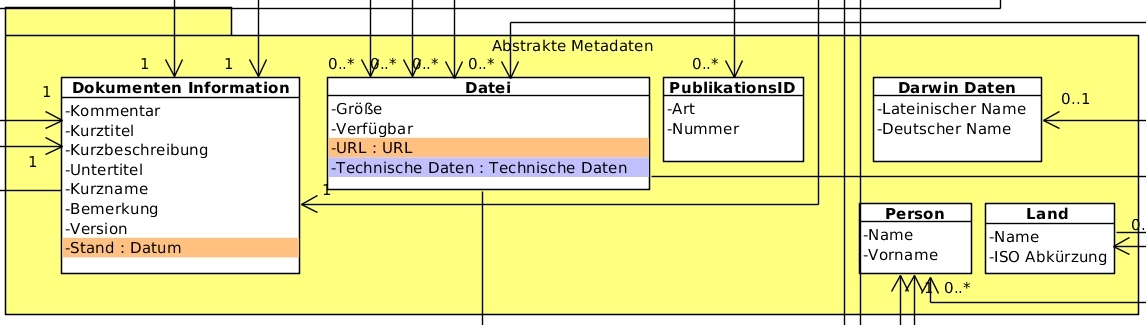
\includegraphics[width=15cm]{Bilder/Datenmodell/Package-Abstrakte-Metadaten.jpg}
\caption{Package Abstrakte Metadaten}
\label{Package Abstrakte Metadaten}
\centering
\end{figure}

\subsubsection{Standard Metadaten}
Das Package \texttt{Standard Metadaten} enth\"alt Datensammlungen f\"ur Standard Metadaten. Im speziellen sind das \texttt{Inspire} und \texttt{Dublin Core}, welche in de Abschnitten \ref{INSPIRE} und \ref{Dublin Core} schon analysiert wurden.

Die Datensammlungen im Package enthalten keine eigenen Attribute, sondern verweisen legiglich auf die ihn ihnen enthaltenen Datensammlungen, welche im Abschnitt \ref{Abstrakte Standard Metadaten} genauer beschrieben werden. Ausnahme hierbei ist das Datum, welches \texttt{Inspire} inne hat und einen Verweis darstellt. (siehe Abschnitt \ref{Grundlegenden Daten})

\begin{figure}[!ht]
\centering
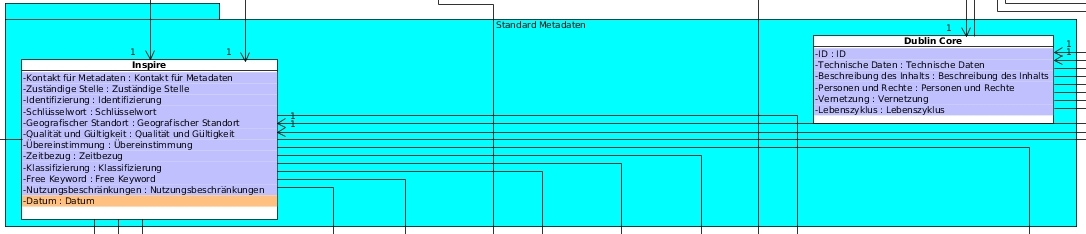
\includegraphics[width=16cm]{Bilder/Datenmodell/Package-Standard-Metadaten.jpg}
\caption{Package Standard Metadaten}
\label{Package Standard Metadaten}
\centering
\end{figure}

\subsubsection{Abstrakte Standard Metadaten}\label{Abstrakte Standard Metadaten}
\texttt{Abstrakte Standard Metadaten} ist das Package, in welchem alle Datensammlungen zu finden sind, die in den \texttt{Standard Metadaten} verwendet werden.

In Abbildung \ref{Package Abstrakte Standard Metadaten Teil 1} sind die Datensammlungen zu sehen, welche bei \ac{INSPIRE} Verwendung finden. Sie werden an keiner anderen Stelle refrenziert, da die \texttt{Inspire}-Datensammlung in den jeweiligen Obersammlungen anzutreffen ist. (siehe Abschnitt \ref{FADO Metadaten} - \ref{ICT-ENSURE Metadaten} und Abbildung \ref{Fado Modell} - \ref{ICT-ENSURE Modell})

In der Datensammlung \texttt{Kontakt f\"ur Metadaten} sind die Attribute \texttt{Name der Stelle} und \texttt{EMail Adresse} vorhanden, mit denen der Ansprechpartner der Datei angegeben wird. \"Uber \texttt{Zust\"andige Stelle} wird mit dem Attribut \texttt{Funktion der Stelle} und dem Verweis \texttt{Zust\"andige Stelle} die Stelle, welche die Datei ver\"offentlicht hat genauer beschrieben.

\texttt{Identifizierung} gibt mit den Attributen \texttt{Ressourcenbezeichnung}, \texttt{Ressourcen\"uberblick}, \texttt{Ressourcenverweis} und \texttt{Ressourcensprache} genauer an. Zus\"atzlich lassen sich \texttt{Bezeichner} einf\"ugen. Alle Attribute sind Freitexte \"und k\"onnen von der jeweiligen "`Stelle"' die die Datei ver\"offentlicht vergeben werden. Einzig \texttt{Bezeichner} und \texttt{Ressourcensprache} sind Verweise und werden im Abschnitt \ref{Grundlegenden Daten} genauer beschrieben.

\texttt{Zeitbezug} enth\"alt verschiedene Daten, welche auf die Sammlung \texttt{Datum} siehe Abschnitt \ref{Grundlegenden Daten} verweisen. Im spezielle sind das \texttt{Erstellungsdatum}, \texttt{Datum der Ver\"offentlichung} und \texttt{Datum der letzten \"Anderung}. Zus\"atzlich enth\"alt die Sammlung noch eine Verweis auf \texttt{Zeiliche Ausdehnung}, welche im Abschnitt \ref{Grundlegenden Daten} beschrieben ist.

Die Datensammlung \texttt{Klassifizierung} enth\"alt eine \texttt{Themenkategorie}, welche vorgegeben ist und zum Beispiel im Editor f\"ur \ac{INSPIRE} zu finden sind\footnote{\url{http://inspire-geoportal.ec.europa.eu/editor/}}.

Schl\"usselw\"orter sind in \ac{INSPIRE} fest vorgegeben und k\"onnen ebenfalls im Editor der \ac{EU} eingesehen werden. Diese Schl\"usselw\"orter werden im Model in der Datensammlung \texttt{Schl\"usselwort} angegeben.

Zus\"atzlich zu den vorgegeben Schl\"usselw\"ortern bietet \ac{INSPIRE} auch die M\"oglichkeit eigene zu erstellen. Im Metadatenmodell ist dies in der Datensammlung \texttt{Free  Keyword} abgebildet. Diese enth\"alt zum einen den Wert des Schl\"ussels und einen Verweis \texttt{Herkunft des Vokabulars}, welcher im Abschnitt \ref{Grundlegenden Daten} genauer beschrieben wird.

Die Datensammlung \texttt{Gegografischer Standort} beinhaltet Attribute f\"ur die vier Koordinaten und zwar \texttt{N Breitengrad}, \texttt{E L\"angengrad}, \texttt{S Breitengrad} und \texttt{W L\"angengrad}. Hierbei werden logischer weise zur Standortbeschreibung immer nur zwei ben\"oigt. Zus\"atzlich gibt ein Attribut das Land bzw. die L\"ander (\texttt{Countries}) und den Ort (\texttt{Bezeichnung}) an.

\texttt{Qualit\"at und G\"ultigkeit} das Freitext-Attribut \texttt{Herkunft} und den Verweis \texttt{R\"aumliche Aufl\"osung} welches im Abschnitt \ref{Grundlegenden Daten} genauer beschrieben wird.

\texttt{Nutzungsbeschr\"ankungen} enth\"alt die Freitext-Attribute \texttt{Bedingungen f\"ur Zugang} und \texttt{Beschr\"ankung des \"o\"ofentlichen Zugangs}. Au\ss{}erdem ist ein Verweis auf die Lizenz angegeben, welcher im Abschnitt \ref{Urheber Metadaten} beschrieben wird.

\texttt{\"Ubereinstimmung} ist eine Datensammlung f\"ur die Quellenangabe. Hierbei wird die Quelle im Attribut \texttt{Specifications} angegeben. Zus\"atzlich dazu ist ein Attribut \texttt{Grad} angegeben, welche beinhaltet ob die Quelle konform ist oder nicht. \"Uber den Verweis \texttt{Datum mit Typ} wird angegeben, von wann die Quelle ist. (siehe Abschnitt \ref{Grundlegenden Daten})

\begin{figure}[!ht]
\centering
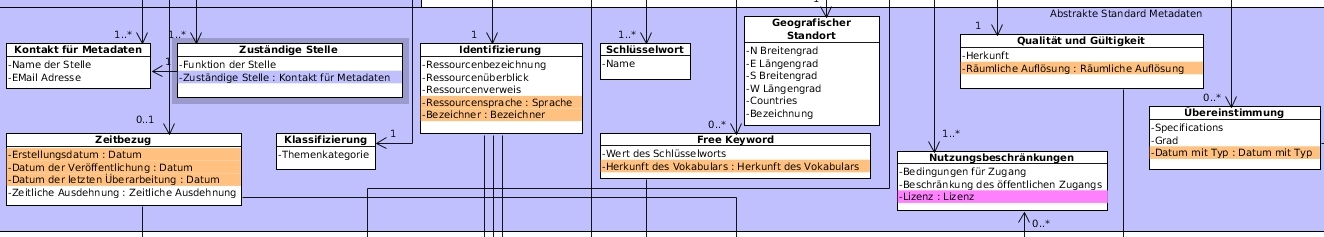
\includegraphics[width=16cm]{Bilder/Datenmodell/Package-Abstrakte-Metadaten-Teil1.jpg}
\caption{Package Abstrakte Standard Metadaten Teil 1 \ac{INSPIRE}}
\label{Package Abstrakte Standard Metadaten Teil 1}
\centering
\end{figure}

In Abbildung \ref{Package Abstrakte Standard Metadaten Teil 2} sind die Datensammlungen aufgezeigt, welche "`Dublin Core"' verwendet. Diese befinden sich ebenfalls im Package \texttt{Abstrakte Standard Metadaten}. "`Dublin Core"' wurde im Abschnitt \ref{Dublin Core} schon analysiert und nun im Modell verwendet.

\texttt{ID} gibt mit dem Attribut \texttt{Identifier} eine eindeutige ID des Dokuments an, welche im System einmalig vergeben wird. \"Uber diese ID sollen sp\"ater Verweise m\"oglich sein.

Die Sammlung \texttt{Technische Daten} beinhaltet die Attribute \texttt{Format} und \texttt{Typ}. Zus\"atzlich wird ein Verweis auf eine \texttt{Sprache} gemacht (siehe Abschnitt \ref{Grundlegenden Daten}). \"Uber diese Felder wird eine "`reale"' Datei genauer beschrieben.

Die Beschreibung des Inhalts wird mit der gleichnamigen Datensammlung \texttt{Beschreibung des Inhalts} umgesetzt. Hierf\"ur stehen die Attribute \texttt{Titel}, \texttt{Thema}, \texttt{Reichweite} und \texttt{Beschreibung} zur Verf\"ugung.

\texttt{Personen und Rechte} hat die beiden Attribute \texttt{Rechteverwerter} und \texttt{Herkunft}. Zus\"atzlich sind die beiden Verweise \texttt{Urheber} udn \texttt{Herausgeber} zu finden, welche im Abschnitt \ref{Urheber Metadaten} genauer erl\"autert werden. Der Verweis \texttt{Mitarbeiter} zeigt auf die Datensammlung Person und ist im Abschnitt \ref{Abstrakte Metadaten} aufgef\"uhrt.

Mit der Datensammlung \texttt{Vernetzung} kommen die vier Attribute \texttt{Quelle}, \texttt{Verweis}, \texttt{Zielgruppe} und \texttt{Lehrmethode}. Die Felder \texttt{Quelle}, \texttt{Verweis} und \texttt{Zielgruppe} sind eindeutig und werden an dieser Stelle nicht weiter erl\"autert. Das Attribut \texttt{Lehrmethode} gibt an, mit welcher Lehrmethode sich die Daten am besten vermitteln lassen, beziehungsweise wie sie vermittelt werden.

\texttt{Lebenszyklus} gibt einen Verweis auf ein Datum (siehe Abschnitt \ref{Grundlegenden Daten}) und ein Attribut \texttt{Zustand}, mit dem sich beschreiben l\"asst um was f\"ur ein Datum es sich handelt.

\begin{figure}[!ht]
\centering
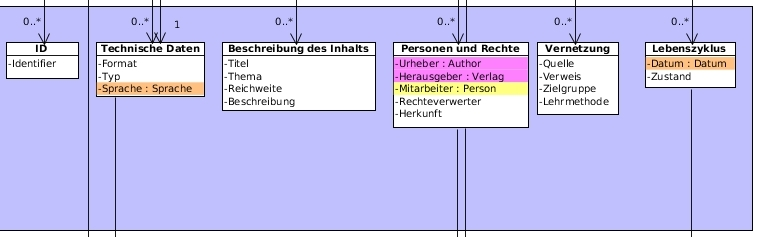
\includegraphics[width=11cm]{Bilder/Datenmodell/Package-Abstrakte-Metadaten-Teil2.jpg}
\caption{Package Abstrakte Standard Metadaten Teil 2 "`Dublin Core"'}
\label{Package Abstrakte Standard Metadaten Teil 2}
\centering
\end{figure}

\FloatBarrier
\subsubsection{Grundlegenden Daten} \label{Grundlegenden Daten}
Das Package \texttt{Grundlegende Daten}, welches in Abbildung \ref{Package Grundlegende Daten} zu sehen ist, beinhaltet grundlegende Datensammlungen und wird daher an vielen Stellen im Modell verwendet. 

Die Datensammlung \texttt{Datum} enth\"alt die eindeutigen Attribute \texttt{Tag}, \texttt{Monat} und \texttt{Jahr}. Die Sammlung wird vielfach verwendet, wovon auch die Pfeile zur Sammlung in der Abbildung \ref{Package Grundlegende Daten} zeugen.

\texttt{Sprache} ent\"alt lediglich das eine Attribut \texttt{Name}, in welchem die entsprechende Sprache angegeben wird.

\texttt{URL} enth\"alt ebenfalls nur ein Attribut \texttt{Link}, welches einen internen oder externen Link repr\"asentiert.

Die Sammlung \texttt{Bezeichner} enth\"alt die Attribute \texttt{Code} und \texttt{Namensraum}. Im \ac{INSPIRE}-Standard gibt der \texttt{Code} eine eindeutige ID an, welche durch den \texttt{Namensraum} eingeschr\"ankt und genauer spezifiziert wird. (siehe Abschnitt \ref{Abstrakte Standard Metadaten})

Mit der Datensammlung \texttt{Herkunft des Vokabulars} wird angegeben aus welchem Vokabular das frei gew\"ahlte Schl\"usselwort stammt. Zus\"atzlich wird ein Datum verlangt, wann das Schl\"usselwort entsand, ge\"andert oder ver\"offentlicht wurde, was mit Hilfe des Attributs \texttt{Datentyp} geschieht.

\texttt{Zeitliche Ausdehnung} ist eine Sammlung, welche ein \texttt{Anfangsdatum} und ein \texttt{Enddatum} als Verweis auf die Sammlung \texttt{Datum} enth\"alt.

\texttt{R\"aumliche Aufl\"osung} enth\"alt drei Attribute, und zwar \texttt{\"Aquivalenter Ma\ss{}stab}, \texttt{Aufl\"osungsabstand} und \texttt{L\"angeneinheit}. Sie werden ben\"otigt um eine genaue geografische Aufl\"osung des Standortes zu gew\"ahrleisten.


\begin{figure}[!ht]
\centering
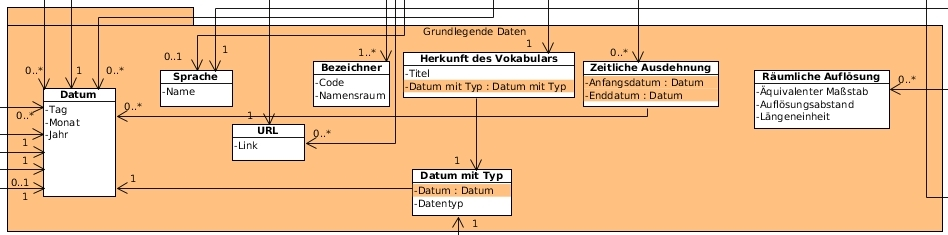
\includegraphics[width=16cm]{Bilder/Datenmodell/Package-Grundlegende-Daten.jpg}
\caption{Package Grundlegende Daten}
\label{Package Grundlegende Daten}
\centering
\end{figure}

\subsubsection{Urheber Metadaten} \label{Urheber Metadaten}
Im Package \texttt{Urheber Metadaten} sind Datensammlungen zusammengefasst, welche sich mit der Urheberschaft von Dateien befassen.

\texttt{Verlag} enth\"alt die Attribute \texttt{Name} und \texttt{Ort}. Zus\"atzlich einen Verweis auf die Datensammlung \texttt{Land} aus dem Package \texttt{Abstrakte Metadaten} welches im Abschnitt \ref{Abstrakte Metadaten} beschrieben ist. Au\ss{}erdem ist ein Verweis auf eine \texttt{Lizenz} zu finden, welche sich im selben Package befindet.

Die Datensammlung \texttt{Lizenz} hat das Attribut \texttt{Lizenzart}, in welchem der Lizenzname festgehalten wird. Au\ss{}erdem ist ein Verweis auf eine \texttt{Person} vorhanden, welche den Lizenzinhaber ausweist. (siehe Abschnitt \ref{Abstrakte Metadaten})

Der \texttt{Autor} enth\"alt das Attribut Institution und die Verweise auf \texttt{Person} und \texttt{Land}, welche zum Package \texttt{Abstrakte Metadaten} geh\"oren und im Abschnitt \ref{Abstrakte Metadaten} beschrieben sind.

Das Attribut \texttt{Institution} k\"onnte weiter aufgeschl\"usselt werde, dies ist jedoch nicht sinnvoll da die Informationen von den Systemen nicht verarbeitet werden.

\begin{figure}[!ht]
\centering
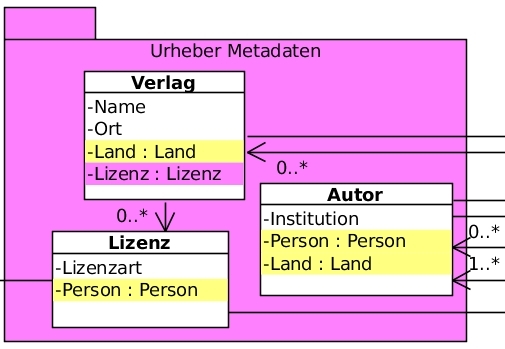
\includegraphics[width=6cm]{Bilder/Datenmodell/Package-Urheber-Metadaten.jpg}
\caption{Package Urheber Metadaten}
\label{Package Urheber Metadaten}
\centering
\end{figure}

\subsection{Metadatenmapping im neuen Modell}\label{Metadatenmapping}
Da sich durch das Zusammenfassen und das Aufstellen eines \"ubergreifenden Modells der Metadaten einige Bezeichnungen von Attribute ge\"andert haben, wird in diesem Abschnitt nun das Mapping zwischen dem alten und neuen Modell beschrieben. Hierf\"ur werden die Metadaten der einzelnen Systeme aufgeschl\"usselt.

\subsubsection{Metadatenmapping FADO}\label{Fado Mapping}
Im folgenden Abschnitt sind die Metadaten des \ac{FADO}-Systems in Tabellenform aufgelistet. Die Auflistung der Metadaten und ihrer Wertebereiche ist im Anhang \ref{Metadaten der LUBW Fachsysteme} zu finden.

In der dargestellten Tabellen \ref{Fado Mapping Urteile}, \ref{Fado Mapping Forschungsvorhaben} und \ref{Fado Mapping Berichte} sind die alten Namen neben den neuen Namen zu finden. Die zus\"atzliche dritte Spalte listet auf in welcher Datensammlung die Attribute zu finden sind.

\begin{table}[!ht]
\begin{center}
\begin{tabular}{|l|l|l|}
\hline
Alt: & Neu: & Klasse: \\ \hline
Fachsystem & Fachsystem & FADO-Metadaten \\ \hline
ID & ID & ID \\ \hline
Titel & Titel & Beschreibung des Inhalts \\ \hline
Tenor & Tenor & Urteils Metadaten \\ \hline
Kommentar & Beschreibung & Beschreibung des Inhalts \\ \hline
Orientierungssatz & Orientierungssatz & Urteils Metadaten \\ \hline
Norm & Norm & Urteil \\ \hline
Leitsatz & Leitsatz & Urteils Metadaten \\ \hline
Gericht & Gericht & Urteil \\ \hline
Entscheidungsform & Entscheidungsform & Urteil \\ \hline
Entscheidungsdatum & Entscheidungsdatum & Urteils Metadaten \\ \hline
Aktenzeichen & Aktenzeichen & Urteils Metadaten \\ \hline
Vorgericht & Vorgericht & Urteils Metadaten \\ \hline
Nachgericht & Nachgericht & Urteils Metadaten \\ \hline
Sachverhalt & Sachverhalt & Urteils Metadaten \\ \hline
Gr�nde & Gr�nde & Urteils Metadaten \\ \hline
Unsichtbar & Unsichtbar & FADO-Metadaten \\ \hline
Ausblenden & Ausblenden & FADO-Metadaten \\ \hline
\end{tabular}
\caption{Mapping der FADO Attribute f�r Urteile}
\label{Fado Mapping Urteile}
\end{center}
\end{table}

\begin{table}[htbp]
\begin{center}
\begin{tabular}{|l|l|l|}
\hline
Alt: & Neu: & Klasse: \\ \hline
Fachsystem & Fachsystem & FADO-Metadaten \\ \hline
ID & ID & ID \\ \hline
Title & Titel & Beschreibung des Inhalts \\ \hline
Kurzbeschreibung & Kurzbeschreibung & Dokumenten Information \\ \hline
Kommentar & Kommentar & Dokumenten Information \\ \hline
F�rderbereich & F�rderbereich & Forschungsvorhaben \\ \hline
Beginn & Beginn & Forschungsvorhaben \\ \hline
Ende & Ende & Forschungsvorhaben \\ \hline
Projektnummer & Projektnummer & Forschungsvorhaben \\ \hline
F�rderkennzeichen & F�rderkennzeichen & Forschungsvorhaben \\ \hline
Unsichtbar & Unsichtbar & FADO-Metadaten \\ \hline
Ausblenden & Ausblenden & FADO-Metadaten \\ \hline
\end{tabular}
\caption{Mapping der FADO Attribute f�r Forschungsvorhaben}
\label{Fado Mapping Forschungsvorhaben}
\end{center}
\end{table}

\FloatBarrier
Die Attribute \texttt{HTML-Datei}, \texttt{PDF-Datei}, \texttt{Weitere Datei} und \texttt{Format dieser Datei} sind am interssantesten, da sie komplett durch die Datensammlung \texttt{Datei} ersetzt werden, wie in der Tabelle \ref{Fado Mapping Berichte} zu sehen ist.

Da w\"ahrend der Bearbeitung der Metadaten eine neue Version des \ac{FADO}-Systems verabschiedet wurde ergaben sich einige \"Anderungen in den Metadaten. Hierdurch entfallen die Attribut \texttt{Seiten (von-bis)}, \texttt{Shoprelevant}, \texttt{Shoplink} und \texttt{Preis} ersatzlos.

\begin{table}[htbp]
\begin{center}
\begin{tabular}{|l|l|l|}
\hline
Alt: & Neu: & Klasse: \\ \hline
Fachsystem & Fachsystem & FADO-Metadaten \\ \hline
ID & ID & ID \\ \hline
Titel & Titel & Beschreibung des Inhalts \\ \hline
Kurzbeschreibung & Kurzbeschreibung & Dokumenten Information \\ \hline
Kommentar & Kommentar & Dokumenten Information \\ \hline
Kurztitel & Kurztitel & Dokumenten Information \\ \hline
Untertitel & Untertitel & Dokumenten Information \\ \hline
Fachthema & Thema & Beschreibung des Inhalts \\ \hline
Herausgeber & Herausgeber & Personen und Rechte \\ \hline
Redaktion & Redaktion & Bibliographische Angaben \\ \hline
Version & Version & Dokumenten Information \\ \hline
Stand & Stand & Dokumenten Information \\ \hline
Seitenzahl & Seitenzahl & Literatur Metadaten \\ \hline
Seite (von-bis) & ENTF�LLT & ENTF�LLT \\ \hline
Reihe & Reihe & Literatur Metadaten \\ \hline
Bandnummer & Bandnummer & Literatur Metadaten \\ \hline
ISSN & PublikationsID & Literatur Metadaten \\ \hline
ISBN & PublikationsID & Literatur Metadaten \\ \hline
Preis & ENTF�LLT & ENTF�LLT \\ \hline
Medium & Format & Technische Daten \\ \hline
Shoprelevant & ENTF�LLT & ENTF�LLT \\ \hline
Shoplink & ENTF�LLT & ENTF�LLT \\ \hline
HTML-Datei & Datei & Bibliographische Angaben \\ \hline
PDF-Datei & Datei & Bibliographische Angaben \\ \hline
Weitere Datei & Datei & Bibliographische Angaben \\ \hline
Format dieser Datei & Format & Technische Daten \\ \hline
Unsichtbar & Unsichtbar & FADO-Metadaten \\ \hline
Ausblenden & Ausblenden & FADO-Metadaten \\ \hline
\end{tabular}
\end{center}
\caption{Mapping der FADO Attribute f�r Berichte}
\label{Fado Mapping Berichte}
\end{table}

\FloatBarrier
\subsubsection{Metadatenmapping DRS}\label{DRS Mapping}
Wie eben schon im Abschnitt \ref{Fado Mapping} erkl\"art, wurden die Namen der Attribute auch f\"ur das \ac{DRS} ge\"andert. Die alte Bezeichnung ist in der linken Spalte, der neue Name im Modell in der mittleren Spalte und die zugeh\"orige Datensammlung in der rechten Spalte, in der Tabelle \ref{DRS Mapping Tabelle}, zu finden. 

Die Auflistung der Metadaten und ihrer Wertebereiche ist im Anhang \ref{Anhang Metadaten des DRS} zu finden.

\begin{table}[htbp]
\begin{center}
\begin{tabular}{|l|l|l|}
\hline
Alt: & Neu: & Klasse: \\ \hline
G�ltigkeit & G�ltigkeit / G�ltigkeitszusatz & DRS-Metadaten \\ \hline
Titel & Titel & Beschreibung des Inhalts \\ \hline
Aktenzeichen & Aktenzeichen & DRS-Metadaten \\ \hline
Kurz-Titel & Kurztitel & Dokumenten Information \\ \hline
Dokumentart & Dokumentart & Ablage \\ \hline
Herausgeber & Herausgeber & Personen und Rechte \\ \hline
Erscheinungsort & Herkunft & Personen und Rechte \\ \hline
Handbuch & Handbuch & Ablage \\ \hline
Kapitel & Kapitel & Ablage \\ \hline
Fundstelle & Fundstelle & Ablage \\ \hline
Fassung & Fassung & Datum Rechtsvorschriften \\ \hline
�nderung & �nderung & Datum Rechtsvorschriften \\ \hline
Gr��e & Gr��e & Datei \\ \hline
Formate & Format & Technische Daten \\ \hline
\end{tabular}
\end{center}
\caption{Mapping der DRS Attribute }
\label{DRS Mapping Tabelle}
\end{table}


\subsubsection{Metadatenmapping Bildarchiv}\label{Bildarchiv Mapping}
Auch die Metadaten des Bildarchivs mussten zum Teil umbenannt werden um ein einheitliches Modell zu erstellen. Wie in dem Abschnitten \ref{Fado Mapping} und \ref{DRS Mapping} ist die Tabelle \ref{Bildarchiv Mapping Tabelle} nach dem gleichen Muster aufgebaut. Links die alten Namen, in der Mitte die neuen Namen und Rechts die zugeh\"orige Datensammlung.

Im alten Attribut \texttt{Bemerkung} steht der Name des biologischen Objekts in deutsch und lateinisch, dies wird im neuen System durch die Datensammlung \texttt{Darwin Daten} getrennt verwaltet und gespeichert, was ein Abrufen der einzelnen Attribute deutlich vereinfacht.

Die Auflistung der Metadaten und ihrer Wertebereiche ist im Anhang \ref{Anhang Metadaten des Bildarchivs} zu finden.

\begin{table}[htbp]
\begin{center}
\begin{tabular}{|l|l|l|}
\hline
Alt: & Neu: & Klasse: \\ \hline
Objektart & Thema & Beschreibung des Inhalts \\ \hline
Objektname & Lateinischer Name & Darwin Daten \\ \hline
ID & ID & ID \\ \hline
URL & URL & Datei \\ \hline
Dateityp & Format & Technische Daten \\ \hline
Name & Name & Bildarchiv-Metadaten \\ \hline
Kurzname & Kurzname & Bildarchiv-Metadaten \\ \hline
Erstellt am & Datum & Lebenszyklus \\ \hline
Autor & Urheber & Personen und Rechte \\ \hline
Besitzer & Rechteverwerter & Personen und Rechte \\ \hline
Bemerkung & Darwin Daten & Darwin Daten \\ \hline
\end{tabular}
\end{center}
\caption{Mapping der Bildarchiv Attribute}
\label{Bildarchiv Mapping Tabelle}
\end{table}


\subsubsection{Metadatenmapping ICT-ENSURE}
Die Tabelle \ref{ICT-ENSURE Mapping Tabelle} folgt dem Schema aus den Abschnitten \ref{FADO Metadaten}, \ref{DRS Mapping} und \ref{Bildarchiv Mapping}.

Dadurch das die Metadaten der \ac{ICT-ENSURE} urspr\"unglich in einer relationalen Datenbank abgelegt wurden, entfallen hier nun einige Attribute, \"uber die f\"urher die Relationen abgebildet wurden.

Die Auflistung der Metadaten und ihrer Wertebereiche ist im Anhang \ref{Metadaten der ICT-ENSURE} zu finden.

\begin{table}[htbp]
\begin{center}
\begin{tabular}{|l|l|l|}
\hline
Alt: & Neu: & Klasse: \\ \hline
Editor & Konferenzauthor & Konferenz \\ \hline
Publisher & Herausgeber & Personen und Rechte \\ \hline
Year of Publishing & Datum & Lebenszyklus \\ \hline
ISBN & PublikationsID & Literatur Metadaten \\ \hline
Conferenc & Konferenztitel & Konferenz \\ \hline
Editor & Urheber & Personen und Rechte \\ \hline
Publisher & ENTF�LLT & ENTF�LLT \\ \hline
Year of Pblishing & ENTF�LLT & ENTF�LLT \\ \hline
ISBN & ENTF�LLT & ENTF�LLT \\ \hline
Conferenc & Thema & Beschreibung des Inhalts \\ \hline
Editor & Urheber & Personen und Rechte \\ \hline
Name & Titel & Beschreibung des Inhalts \\ \hline
Konferenz & ENTF�LLT & ENTF�LLT \\ \hline
Kapitel & ENTF�LLT & ENTF�LLT \\ \hline
Author & ENTF�LLT & ENTF�LLT \\ \hline
Dateityp & Format & Technische Daten \\ \hline
Titel & ENTF�LLT & ENTF�LLT \\ \hline
Sprache & Ressourchensprache & Sprache \\ \hline
Beginn Seite & Beginn Seite & Literatur Metadaten \\ \hline
End Seite & End Seite & Literatur Metadaten \\ \hline
Schl�sselw�rter & Sch�sselwort / Free Keyword & Inspire \\ \hline
Abstract & Abstract & Literatur Metadaten \\ \hline
Volltext & Volltext & Artikel-Metadaten \\ \hline
\end{tabular}
\end{center}
\caption{Mapping der \ac{ICT-ENSURE} Attribute }
\label{ICT-ENSURE Mapping Tabelle}
\end{table}
